\def\customcitkey{Urban2018}\def\absintkey{Cousot1977}


\pagelayout{margin} % Restore margins
\chapter*{Kaobook Template Motivation}
\addcontentsline{toc}{chapter}{Kaobook Template Motivation}

For this manuscript, we have selected the \textsc{Kaobook} class,\sidenote{\rurl{github.com/fmarotta/kaobook}} a template featuring a wide margin specifically designed for writing books and graduate-level theses, based on Ken Arroyo Ohori's doctoral thesis\sidenote{\rurl{3d.bk.tudelft.nl/ken/en/thesis}} and on the \textsc{Tufte}-\LaTeX{} class,\sidenote{\rurl{ctan.org/pkg/tufte-latex}} offering a layout that is both elegant and practical.

\marginnote{\formatmargincitation{\absintkey}}
\begin{marginfigure}
  \centering
  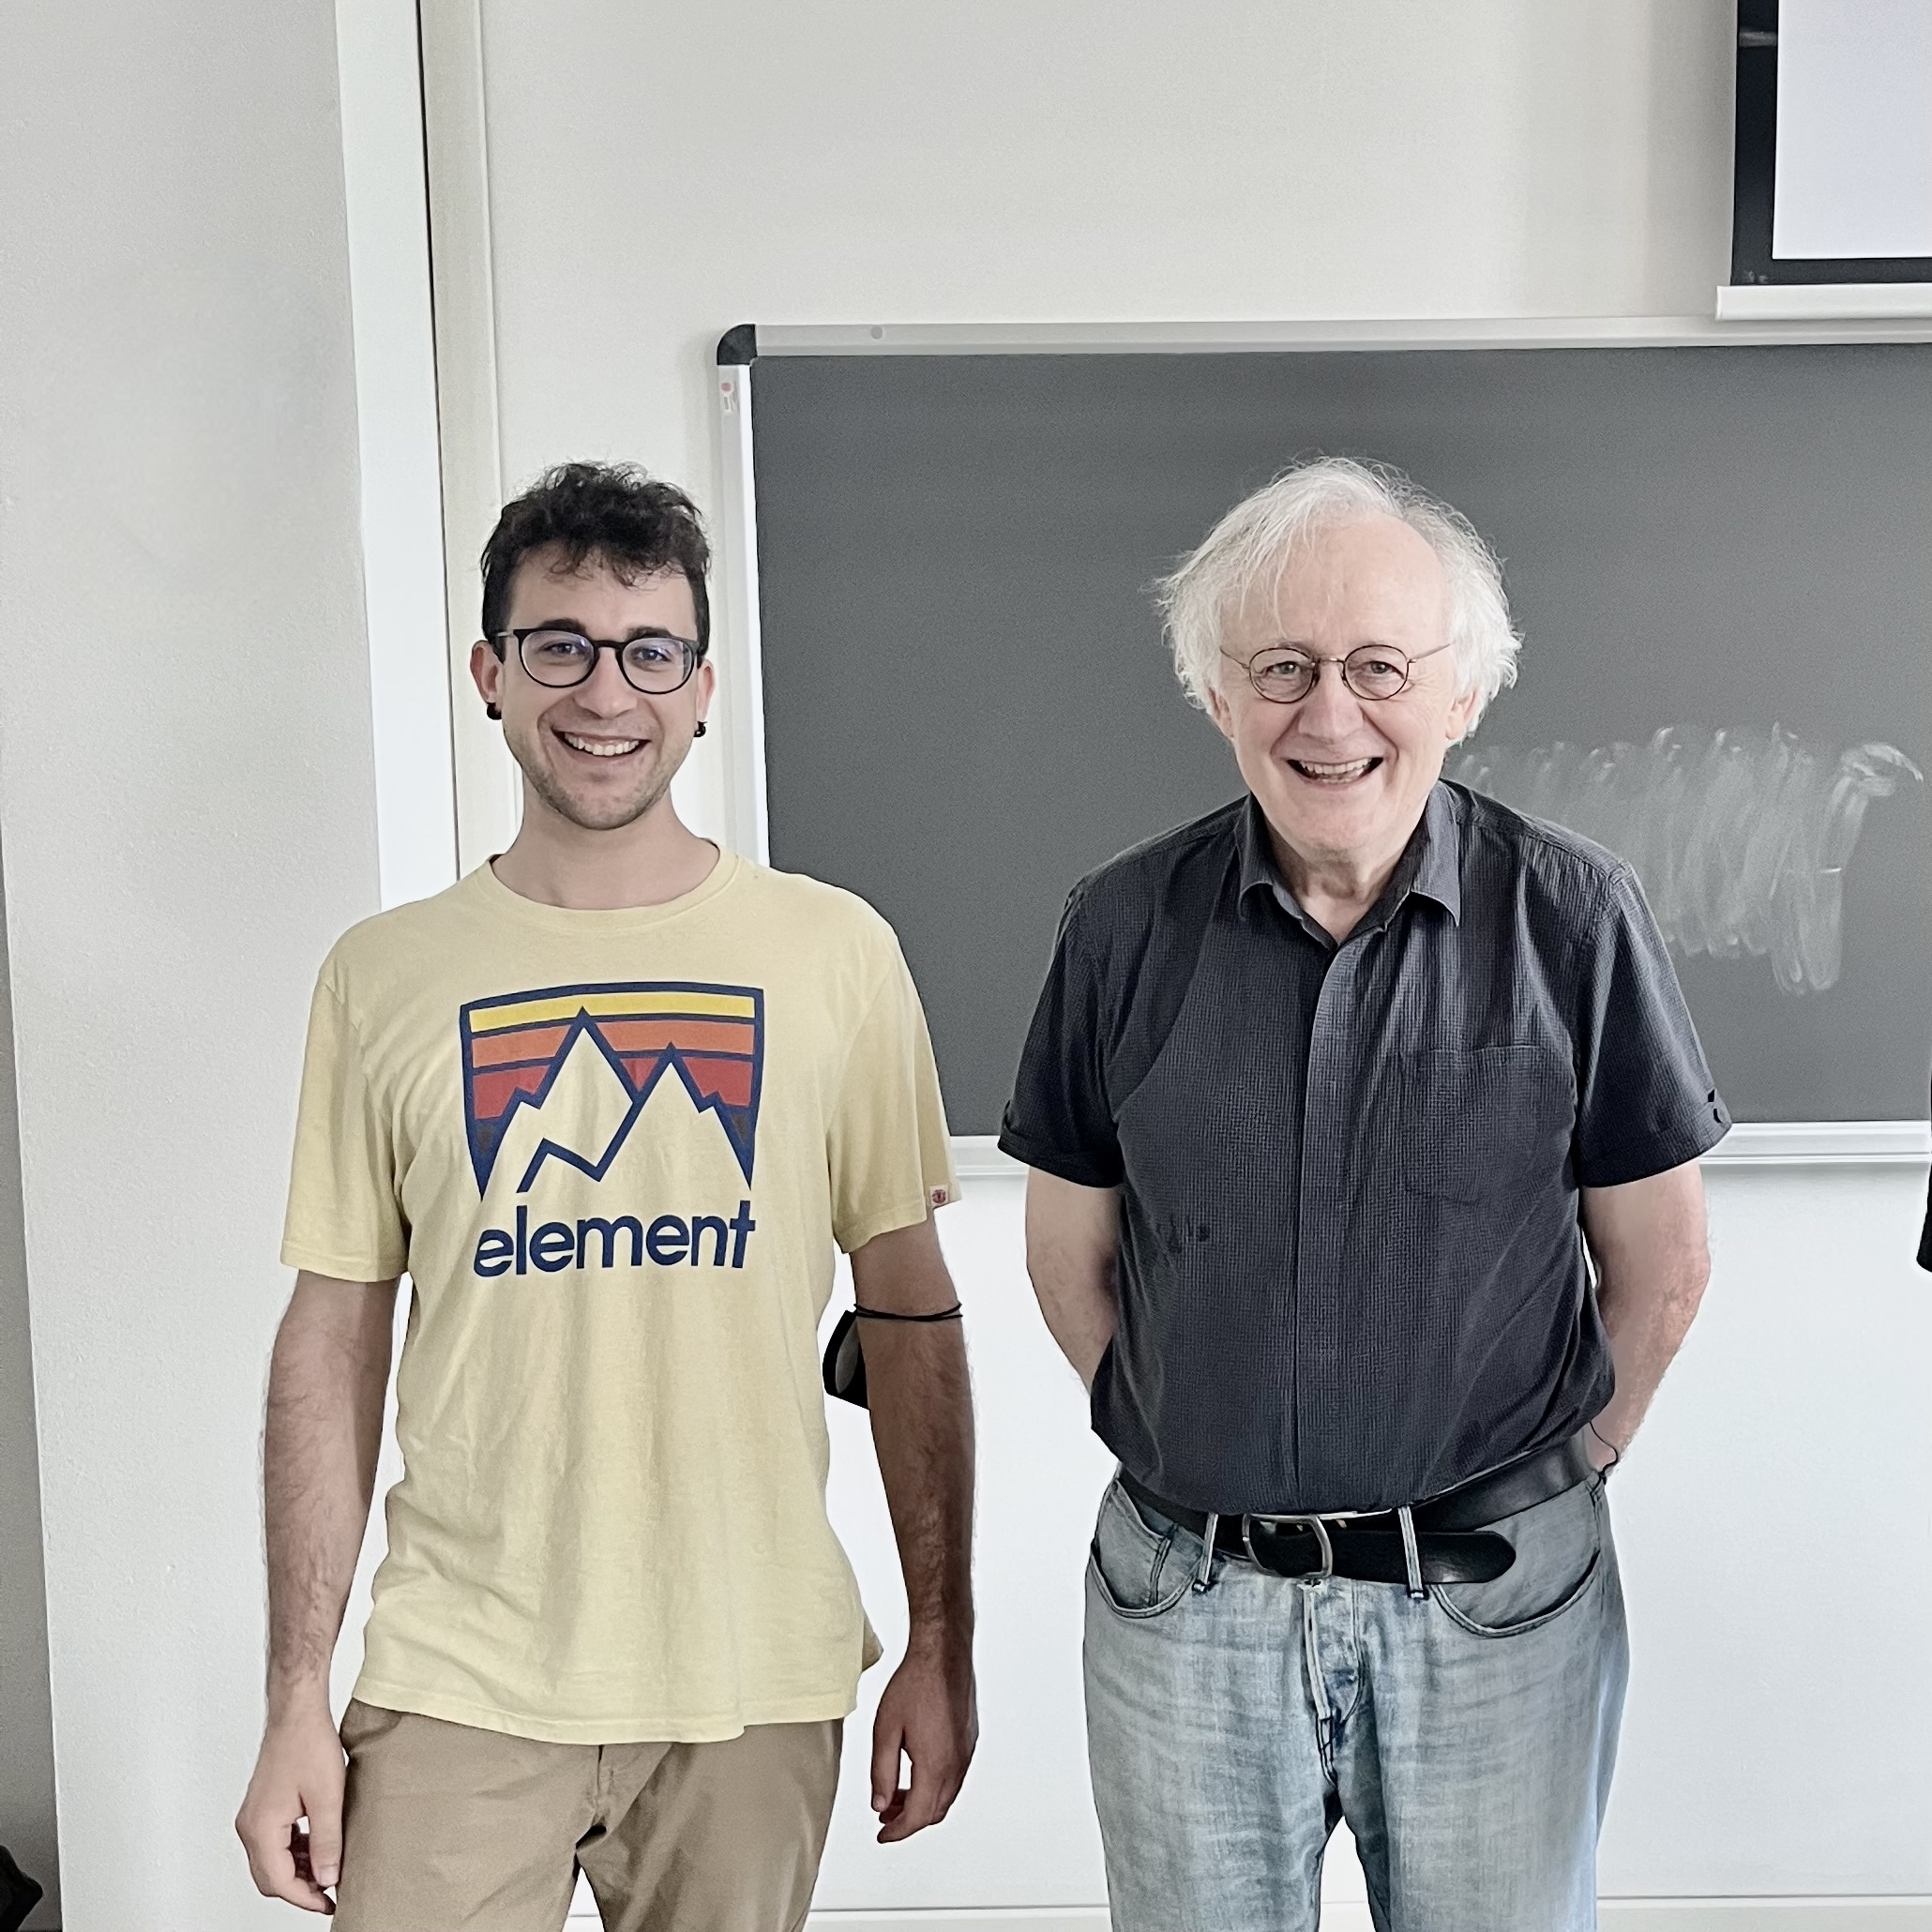
\includegraphics[width=\textwidth]{figures/denis-patrick}
  \caption{Me (left) with Patrick Cousot (right) co-founder of abstract interpretation\cite{\absintkey}.}
  \labfig{denis-patrick}
\end{marginfigure}

\emph{Why the narrow main text column?} It is all about the wide margin: an expansive playground for notes, code snippets, figures, tables, citations, and all those additional details that enhance the narrative, as \reffig{denis-patrick} shows.
This layout lets the main narrative to take the spotlight while all the extra bits are placed in the margin, where they can be easily accessed without disrupting the flow of the text. It is like having a personal assistant handing you the information right when you need it.

With over 200 references in this manuscript, the use of side references becomes a lifesaver.
The hassle of digging back and forth through the bibliography to remember which citation matches \sidecite{\customcitkey} is a thing you will not endure in this thesis.
Speaking of citations, as every computer scientist knows, ``42'' is the answer of Life, the Universe and Everything, according to Douglas Adams' \emph{The Hitchhiker's Guide to the Galaxy}.\sidenote{\rurl{en.wikipedia.org/wiki/Phrases_from_The_Hitchhiker\%27s_Guide_to_the_Galaxy\#The_Answer_to_the_Ultimate_Question_of_Life,_the_Universe,_and_Everything_is_42}}
But for this thesis, the 42nd citation holds even more weight--it is the work, written by my supervisor Caterina Urban in 2018, laid the foundation for the property of input data usage, unifying existing literature on information flow analyses within the framework of abstract interpretation\cite{\absintkey}. In essence, \cite{\customcitkey} inspired my academic journey and the last four years of my life.

The template also allows for brief restatements of definitions and theorems in the margins, linked to their original appearances.
This means you will not flip through the pages up and down this manuscript--once a concept is introduced, it conveniently pops up in the margin whenever relevant again.
Recalling \refdef*{poset} of a \emph{partially ordered set} has never been easier, and for the electronic version of this thesis, you can also click on the title of the margin definition to jump to its original appearance in the text.
This keeps the discussion clear and accessible, which is especially valuable in a complex and detailed work like a PhD thesis. In short:
\begin{center}\itshape
this wide-margin template makes navigating through these pages a bit easier, \\
and hopefully, a bit more enjoyable too.
\end{center}
